\documentclass{beamer}

\usetheme{Madrid}

\title{Simulated Annealing}
\author{Matheus Marinho, Guilherme Freire, Italo Costa}
\date{\today}

\begin{document}

\frame{\titlepage}

\begin{frame}{O que é otimização?}
    \begin{itemize}
        \item Ação ou efeito de otimizar;
        \item Produzir condições apropriadas para o melhor desenvolvimento de algo;
        \item Encontrar a melhor solução dentro de um espaço de soluções;
        \item Processo de busca dos argumentos que resultam no valor extremo de uma ou mais funções que representem o problema.
    \end{itemize}
    \begin{figure}
        \includegraphics[scale = 0.35]{src/Ponto ótimo.drawio.png}
    \end{figure}
\end{frame}

\begin{frame}{Exemplos práticos}
    \begin{itemize}
        \item Busca de caminho mais curto em mapas;
        \item Minimização de custos;
        \item Maximização de lucros;
        \item Design de circuitos;
        \item Planejamento logístico.
    \end{itemize}
\end{frame}

\begin{frame}{Desafios da otimização}
    
\end{frame}

\begin{frame}{Simulated Annealing: Analogia Física}
        O recozimento de metais (também chamado de recristalização) é um processo de alteração
    de propriedades de um material metálico por aquecimento e resfriamento lento.Quando um material é submetido a um processamento a frio, sua estrutura cristalina é
    deformada e surgem vários pontos de tensão. Os cristais deformados têm mais energia que os não
    deformados, por causa da desorganização da estrutura cristalina nas interfaces entre os grãos. Esta
    estruturas são estáveis nesta temperatura, já que os átomos não têm mobilidade suficiente para
    alterar a sua organização cristalina. Havendo oportunidade, os átomos irão se deslocar visando um
    arranjo mais perfeito e regular, de menor energia.
\end{frame}

\begin{frame}{Simulated Annealing: Algoritmo Básico}
    O método de Recozimento Simulado (simulated annealing) é um tipo de método de busca
local de implementação extremamente simples proposto por METROPOLIS et al. (1953), que
perceberam que a natureza faz na verdade a minimização da energia da estrutura cristalina quando o
material é recozido para remover defeitos de sua estrutura atômica. KIRKPATRICK et al. (1983)
estenderam o método de otimização termodinâmica de Metropolis para o problema de otimização
combinatorial.
\end{frame}

\begin{frame}
    \begin{itemize}
        \item O estado do sistema termodinâmico corresponde à solução atual do problema;
        \item A equação de energia para o sistema é a função objetivo;
        \item O estado de referência é análogo ao mínimo global da função;
        \item O que evita o algoritmo de ficar preso em um mínimo local é a seleção adequada da programação do recozimento:
        \begin{itemize}
            \item Temperatura inicial;
            \item Número de iterações do algoritmo com a mesma temperatura;
            \item Estratégia de redução de temperatura;
            \item Definição de uma estrutura de vizinhança.
        \end{itemize}
    \end{itemize}
\end{frame}

\begin{frame}
    A partir de um ponto no espaço de soluções, calcula-se um novo ponto vizinho do atual. 
    Se a energia (valor da função objetivo) é menor neste novo ponto, este passa a ser nosso 
    ponto atual. Se a energia é maior neste novo ponto, ele não é automáticamente descartado. 
    Há uma certa probabilidade de ele ser aceito como o novo ponto atual, e esta probrabilidade 
    é tão maior quanto maior for o parâmetro temperatura ou quanto menor for a diferença de 
    energia entre os dois pontos.
\end{frame}

\begin{frame}
    Queremos reduzir o valor da energia, mas ainda assim aceitamos como nova solução um
ponto que seja pior que o anterior? O motivo para esta aparente contradição é simples: para que se
vá de um mínimo local a um mínimo global da estrutura acessando apenas pontos vizinhos, é
necessário que, pelo menos em alguns pontos ao longo desta trajetória, a energia do sistema
aumente. Em outras palavras, a única maneira de ir de um mínimo local para o mínimo global (ou
para outro mínimo local) é aumentando a energia do sistema.
\end{frame}

\begin{frame}{Redução de temperatura}
    \begin{itemize}
        \item Qualquer função monótona decrescente pode ser usada como função de resfriamento. Uma
        escolha muito usual é a redução linear da temperatura, fazendo $T^{k+1} = \alpha T^k$. O parâmetro $\alpha$ varia tipicamente entre 0,7 e 0,95. Funções exponenciais de resfriamento são também utilizadas na
        literatura da área.
        \item Como uma regra geral, o número de temperaturas
        empregadas ($n_1$) deve ser pequeno – algo entre 10 e 20 costuma ser suficiente. Já o número de
        iterações com a mesma temperatura ($n_2$) deve ser um pouco maior, para que se dê tempo suficiente
        ao algoritmo para buscar o espaço de soluções com aquela temperatura
    \end{itemize}
\end{frame}

\begin{frame}{Critério de aceitação}
    \begin{itemize}
        \item O critério proposto por Metropolis consiste em avaliar a diferença de energia entre a solução
        atual e a nova solução e calcular $\vartriangle \equiv E^{k+1} -E^k$ . Se $\vartriangle$ é negativo, isto significa que a solução atual é
        melhor que a anterior, e esta última é substituída. Se $\vartriangle$ é positivo, a probabilidade de esta solução de
        maior energia substituir a anterior é dada por $p = e ^ {-\frac{\vartriangle}{T}}$.\\
        \item Como implementar este critério probabilístico de aceitação? Primeiramente é sorteado um
        número randômico $r$ a partir de uma distribuição uniforme no intervalo $[0,1]$. Considere que $p$
        representa a probabilidade de a transição para este novo ponto ser aceita. A probabilidade do
        número sorteado $r$ ser menor ou igual do que $p$, também contido no intervalo $[0,1]$, é $(100p)\%$.
        \item  Logo, se $r < p$ a transição é aceita. Do contrário, este ponto é descartado e um novo vizinho do ponto atual é calculado
    \end{itemize}
\end{frame}

\begin{frame}{Estrutura de vizinhança}
    \begin{itemize}
        \item A definição da estrutura de vizinhança é fundamental para a implementação do algoritmo.
        Uma estrutura de vizinhança nada mais é do que uma maneira de calcular uma solução próxima à
        solução anterior. Para um mesmo problema, várias estruturas de vizinhança são cabíveis. A
        vizinhança de um ponto corresponde ao conjunto de todos os pontos que lhe são vizinhos.
        \item Podemos calcular um ponto “vizinho” no plano real de várias maneiras. Poderíamos: (i) somar (ou
        subtrair) uma quantidade fixa $\delta$ em uma ou mais direções; (ii) dar um passo de tamanho $\delta$ em
        alguma direção arbitrária; (iii) selecionar qualquer ponto que diste não mais que $\delta$ do ponto
        anterior.
    \end{itemize}
    \begin{figure}
        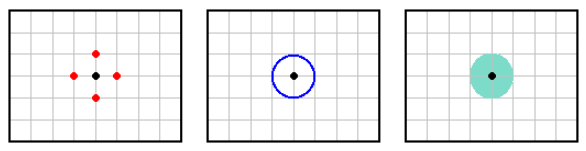
\includegraphics[scale = 0.5]{src/vizinhanca.png}
    \end{figure}
\end{frame}

\begin{frame}{Aspectos de implementação}
    Uma característica do recozimento simulado: não há qualquer garantia de que o último
ponto visitado será o melhor ponto já visitado pelo algoritmo. Uma modificação simples e efetiva
no algoritmo original consiste em registrar em uma variável à parte este melhor resultado
encontrado. Assim, é possível que o seu problema seja resolvido mesmo com uma programação de
recozimento pobre.
\end{frame}

\begin{frame}{Simulated Annealing: Fluxograma}
    \begin{figure}
        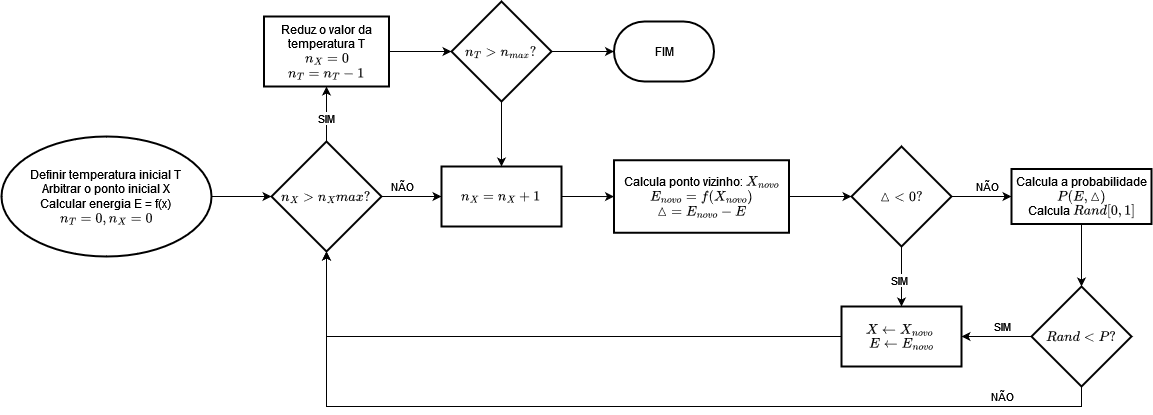
\includegraphics[scale = 0.3]{src/FluxogramaSA.drawio.png}
    \end{figure}
\end{frame}

\begin{frame}{Exemplo ilustrativo}
    Para entender o significado dos parâmetros do método, considere o problema de
minimização da função $F(x)$ apresentada abaixo.
    \begin{equation}
        F(x) = \frac{1}{10000}(x+10)(x+6)(x+5)(x+1)(x-7)(x-10)
    \end{equation}
    \begin{figure}
        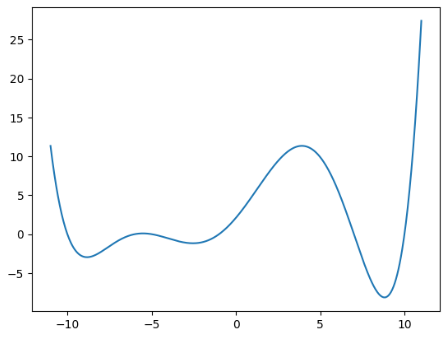
\includegraphics[scale = 0.35]{src/PontoOtimo2.png}
    \end{figure}

Observe que existem mínimos locais em x = -8,834, x = -2,546 e x = 8,817, sendo este
último o mínimo global. A função apresenta máximos locais em x= -5,518 e x = 3,914.
\end{frame}

\begin{frame}{Limitações do algoritmo}
    
\end{frame}

\begin{frame}{Possíveis melhorias}
    
\end{frame}

\begin{frame}{Resumo final}
    
\end{frame}

\begin{frame}
    \begin{center}
        \centering
        \Large{Perguntas?}
    \end{center}
\end{frame}

\end{document}